% Options for packages loaded elsewhere
\PassOptionsToPackage{unicode}{hyperref}
\PassOptionsToPackage{hyphens}{url}
%
\documentclass[
]{article}
\usepackage{lmodern}
\usepackage{amssymb,amsmath}
\usepackage{ifxetex,ifluatex}
\ifnum 0\ifxetex 1\fi\ifluatex 1\fi=0 % if pdftex
  \usepackage[T1]{fontenc}
  \usepackage[utf8]{inputenc}
  \usepackage{textcomp} % provide euro and other symbols
\else % if luatex or xetex
  \usepackage{unicode-math}
  \defaultfontfeatures{Scale=MatchLowercase}
  \defaultfontfeatures[\rmfamily]{Ligatures=TeX,Scale=1}
\fi
% Use upquote if available, for straight quotes in verbatim environments
\IfFileExists{upquote.sty}{\usepackage{upquote}}{}
\IfFileExists{microtype.sty}{% use microtype if available
  \usepackage[]{microtype}
  \UseMicrotypeSet[protrusion]{basicmath} % disable protrusion for tt fonts
}{}
\makeatletter
\@ifundefined{KOMAClassName}{% if non-KOMA class
  \IfFileExists{parskip.sty}{%
    \usepackage{parskip}
  }{% else
    \setlength{\parindent}{0pt}
    \setlength{\parskip}{6pt plus 2pt minus 1pt}}
}{% if KOMA class
  \KOMAoptions{parskip=half}}
\makeatother
\usepackage{xcolor}
\IfFileExists{xurl.sty}{\usepackage{xurl}}{} % add URL line breaks if available
\IfFileExists{bookmark.sty}{\usepackage{bookmark}}{\usepackage{hyperref}}
\hypersetup{
  pdftitle={Second Implementation of QuickPay (2013-2016)},
  hidelinks,
  pdfcreator={LaTeX via pandoc}}
\urlstyle{same} % disable monospaced font for URLs
\usepackage[margin=1in]{geometry}
\usepackage{graphicx}
\makeatletter
\def\maxwidth{\ifdim\Gin@nat@width>\linewidth\linewidth\else\Gin@nat@width\fi}
\def\maxheight{\ifdim\Gin@nat@height>\textheight\textheight\else\Gin@nat@height\fi}
\makeatother
% Scale images if necessary, so that they will not overflow the page
% margins by default, and it is still possible to overwrite the defaults
% using explicit options in \includegraphics[width, height, ...]{}
\setkeys{Gin}{width=\maxwidth,height=\maxheight,keepaspectratio}
% Set default figure placement to htbp
\makeatletter
\def\fps@figure{htbp}
\makeatother
\setlength{\emergencystretch}{3em} % prevent overfull lines
\providecommand{\tightlist}{%
  \setlength{\itemsep}{0pt}\setlength{\parskip}{0pt}}
\setcounter{secnumdepth}{5}
\usepackage{booktabs,longtable,dcolumn} \usepackage{multirow,array} \usepackage{wrapfig,float} \floatplacement{figure}{H}

\title{Second Implementation of QuickPay (2013-2016)}
\author{}
\date{\vspace{-2.5em}Nov 15, 2020}

\begin{document}
\maketitle

\hypertarget{background}{%
\section{Background}\label{background}}

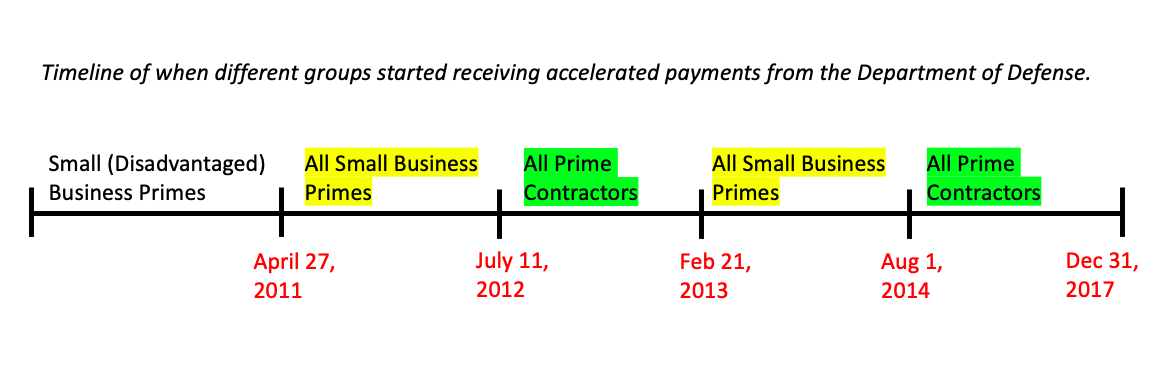
\includegraphics{/Users/vibhutidhingra/Desktop/research/Git:Github/qp_data_and_code/img/policy_timeline.png}

\hypertarget{sample-selection}{%
\section{Sample Selection}\label{sample-selection}}

\begin{itemize}
\item
  Only contracts that were signed on/after March 2013
\item
  Delays measured for quarters March 2013 - March 2016
\item
  Small businesses were receiving faster payments throughout this period
\item
  Payment accelerated to Large Businesses on Aug 1, 2014 (Quarter end
  Sept 30, 2014)
\item
  20 four-digit Naics codes most likely to be treated (per Table A.6 in
  Barrot/Nanda paper)

  \begin{quote}
  This table presents the top 20 and bottom 20 4-digit NAICS industries
  based on treatment, measured as the average quarterly amount of
  eligible government contracts to be performed in a given industry
  between 2009Q1-2011Q1, normalized by quarterly payroll in 2011Q1. --
  Barrot and Nanda 2018
  \end{quote}
\item
  Firm fixed price (type of contract pricing = J)
\item
  Exclude disadvantaged small businesses
\item
  Exclude bundled contracts
\item
  Defense contracts only (agency code = 97)
\item
  Filters applied on DoD data from Fiscal Years 2010-2018 (using
  award-data-archive)
\end{itemize}

\hypertarget{notation}{%
\section{Notation}\label{notation}}

\begin{itemize}
\tightlist
\item
  Project \(i\), Year-Quarter \(t\)
\item
  \(X_i\) denotes project level controls: initial duration, initial
  budget, number of offers received
\item
  \(\mu_t,\theta_{firm},\lambda_{task}\): Year-Quarter, Firm, and
  Product/Service code Fixed effects
\item
  All continuous variables are winsorized at the 5\% level
  \[ Treat_i = \begin{cases} 1, \text{ if project } i \text{ is a large business}\\
  0, \text{ otherwise} \end{cases}\]
  \[ Pre_t = \begin{cases} 1, \text{ if year-quarter } t < \text{ Aug 01, 2014}\\
  0, \text{ otherwise} \end{cases}\]
\end{itemize}

\hypertarget{delays-over-time}{%
\section{Delays over Time}\label{delays-over-time}}

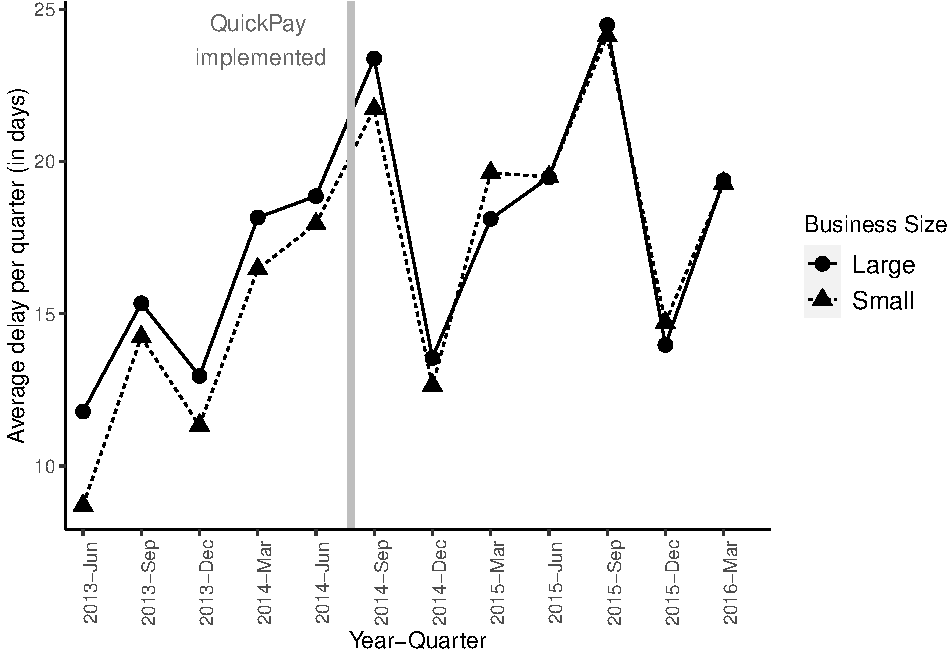
\includegraphics{qp_second_implementation_files/figure-latex/plot-1.pdf}

\hypertarget{parallel-trends-test}{%
\section{Parallel Trends Test}\label{parallel-trends-test}}

\hypertarget{baseline-regressions}{%
\section{Baseline Regressions}\label{baseline-regressions}}

\[ Delay_{it} = \alpha+\beta_0 Treat_i + \beta_1 Pre_t + \beta_2 (Treat_i \times Pre_t) + \epsilon_{it}\]

\[ \begin{aligned} Delay_{it} &=& \alpha+\beta_0 Treat_i + \beta_1 Pre_t + \beta_2 (Treat_i \times Pre_t)\\
&+&  X_i + (Pre_t \times X_i) + \mu_t + \theta_{firm} + \lambda_{task}+ \epsilon_{it}
\end{aligned}\]

\begin{table}[H] \centering 
  \caption{Quickpay 2009-2011} 
  \label{} 
\small 
\begin{tabular}{@{\extracolsep{-2pt}}lccc} 
\\[-1.8ex]\hline 
\hline \\[-1.8ex] 
\\[-1.8ex] & \multicolumn{3}{c}{$Delay_{it}$ (in days)} \\ 
\\[-1.8ex] & (1) & (2) & (3)\\ 
\hline \\[-1.8ex] 
 $Treat_i$ & 0.10 & $-$0.32 & $-$0.44 \\ 
  & (0.25) & (1.00) & (1.02) \\ 
  & & & \\ 
 $Pre_t$ & $-$3.86$^{***}$ &  &  \\ 
  & (0.26) &  &  \\ 
  & & & \\ 
 $Treat_i$x$Pre_t$ & 1.43$^{***}$ & 2.54$^{***}$ & 2.16$^{***}$ \\ 
  & (0.42) & (0.51) & (0.51) \\ 
  & & & \\ 
 Constant & 18.58$^{***}$ &  &  \\ 
  & (0.15) &  &  \\ 
  & & & \\ 
\hline \\[-1.8ex] 
Year-Quarter Fixed Effects & No & Yes & Yes \\ 
Firm Fixed Effects & No & Yes & Yes \\ 
Task Fixed Effects & No & No & Yes \\ 
Duration, Budget, Bids & No & Yes & Yes \\ 
$Pre_t$  x  (Duration, Budget, Bids) & No & Yes & Yes \\ 
Observations & 233,433 & 210,597 & 210,597 \\ 
R$^{2}$ & 0.001 & 0.10 & 0.11 \\ 
Adjusted R$^{2}$ & 0.001 & 0.05 & 0.05 \\ 
\hline 
\hline \\[-1.8ex] 
\textit{Note:}  & \multicolumn{3}{r}{$^{*}$p$<$0.1; $^{**}$p$<$0.05; $^{***}$p$<$0.01} \\ 
 & \multicolumn{3}{r}{Each observation is a project-quarter.} \\ 
 & \multicolumn{3}{r}{SEs are robust and clustered at the project level.} \\ 
\end{tabular} 
\end{table}

\hypertarget{contract-financing}{%
\section{Contract Financing}\label{contract-financing}}

\[ CF_i = \begin{cases} 1, \text{ if project } i \text{ receives contract financing}\\
0, \text{ otherwise} \end{cases}\]

\[ \begin{aligned}
Delay_{it} &=& \alpha+\beta_0 Treat_i + \beta_1 Pre_t + \beta_2 (Treat_i \times Pre_t) \\
&+&\beta_3 CF_i + \beta_4 (CF_i \times Pre_t) + \beta_5 (Treat_i \times Pre_t \times CF_i) \\ 
&+&X_i + (Pre_t \times X_i) + \mu_t + \theta_{firm} + \lambda_{task}+ \epsilon_{it}
\end{aligned}\]

\begin{table}[H] \centering 
  \caption{Effect of Contract Financing: Quickpay 2009-2011} 
  \label{} 
\small 
\begin{tabular}{@{\extracolsep{-2pt}}lccc} 
\\[-1.8ex]\hline 
\hline \\[-1.8ex] 
\\[-1.8ex] & \multicolumn{3}{c}{$Delay_{it}$ (in days)} \\ 
\\[-1.8ex] & (1) & (2) & (3)\\ 
\hline \\[-1.8ex] 
 $Treat_i$ & 0.12 & $-$0.28 & $-$0.39 \\ 
  & (0.24) & (1.00) & (1.02) \\ 
  & & & \\ 
 $Pre_t$ & $-$3.40$^{***}$ &  &  \\ 
  & (0.28) &  &  \\ 
  & & & \\ 
 $Treat_i$x$Pre_t$ & 1.55$^{***}$ & 2.26$^{***}$ & 1.78$^{***}$ \\ 
  & (0.44) & (0.55) & (0.55) \\ 
  & & & \\ 
 $CF_i$ & 6.24$^{***}$ & 0.71 & 0.70 \\ 
  & (0.35) & (0.46) & (0.46) \\ 
  & & & \\ 
 $Pre_t$ x $CF_i$ & $-$3.01$^{***}$ & $-$2.57$^{***}$ & $-$2.48$^{***}$ \\ 
  & (0.75) & (0.86) & (0.86) \\ 
  & & & \\ 
 $Pre_t$ x $CF_i$ x $Treat_i$ & $-$1.20 & 1.68 & 2.42$^{*}$ \\ 
  & (1.10) & (1.25) & (1.26) \\ 
  & & & \\ 
 Constant & 17.70$^{***}$ &  &  \\ 
  & (0.15) &  &  \\ 
  & & & \\ 
\hline \\[-1.8ex] 
Year-Quarter Fixed Effects & No & Yes & Yes \\ 
Firm Fixed Effects & No & Yes & Yes \\ 
Task Fixed Effects & No & No & Yes \\ 
Duration, Budget, Bids & No & Yes & Yes \\ 
$Pre_t$  x  (Duration, Budget, Bids) & No & Yes & Yes \\ 
Observations & 233,433 & 210,597 & 210,597 \\ 
R$^{2}$ & 0.003 & 0.10 & 0.11 \\ 
Adjusted R$^{2}$ & 0.003 & 0.05 & 0.05 \\ 
\hline 
\hline \\[-1.8ex] 
\textit{Note:}  & \multicolumn{3}{r}{$^{*}$p$<$0.1; $^{**}$p$<$0.05; $^{***}$p$<$0.01} \\ 
 & \multicolumn{3}{r}{Each observation is a project-quarter.} \\ 
 & \multicolumn{3}{r}{SEs are robust and clustered at the project level.} \\ 
\end{tabular} 
\end{table}

\hypertarget{receives-financial-aid}{%
\section{Receives Financial Aid}\label{receives-financial-aid}}

\[ FinancialAid = \begin{cases} 1, \text{ if firm receives grants or is a c8A participant}\\
0, \text{ otherwise} \end{cases}\]

\[ \begin{aligned}
Delay_{it} &=& \alpha+\beta_0 Treat_i + \beta_1 Pre_t + \beta_2 (Treat_i \times Pre_t) +\beta_3 FinancialAid \\
&+& \beta_4 (FinancialAid \times Pre_t) + \beta_5 (Treat_i \times Pre_t \times FinancialAid) \\ 
&+&X_i + (Pre_t \times X_i) + \mu_t + \theta_{firm} + \lambda_{task}+ \epsilon_{it}
\end{aligned}\]

\begin{table}[H] \centering 
  \caption{Effect of Grants or C8A Participant: Quickpay 2009-2011} 
  \label{} 
\small 
\begin{tabular}{@{\extracolsep{-2pt}}lccc} 
\\[-1.8ex]\hline 
\hline \\[-1.8ex] 
\\[-1.8ex] & \multicolumn{3}{c}{$Delay_{it}$ (in days)} \\ 
\\[-1.8ex] & (1) & (2) & (3)\\ 
\hline \\[-1.8ex] 
 $Treat_i$ & 0.30 & $-$0.57 & $-$0.67 \\ 
  & (0.25) & (1.01) & (1.02) \\ 
  & & & \\ 
 $Pre_t$ & $-$4.08$^{***}$ &  &  \\ 
  & (0.33) &  &  \\ 
  & & & \\ 
 $Treat_i$x$Pre_t$ & 1.94$^{***}$ & 2.99$^{***}$ & 2.83$^{***}$ \\ 
  & (0.51) & (0.61) & (0.62) \\ 
  & & & \\ 
 $FinancialAid$ & 2.20$^{***}$ & 5.64$^{***}$ & 5.74$^{***}$ \\ 
  & (0.26) & (0.40) & (0.39) \\ 
  & & & \\ 
 $Pre_t$ x $FinancialAid$ & 0.06 & $-$2.64$^{***}$ & $-$2.78$^{***}$ \\ 
  & (0.51) & (0.65) & (0.65) \\ 
  & & & \\ 
 $Pre_t$ x $FinancialAid$ x $Treat_i$ & $-$1.53$^{**}$ & $-$1.22 & $-$1.88$^{**}$ \\ 
  & (0.73) & (0.93) & (0.94) \\ 
  & & & \\ 
 Constant & 17.80$^{***}$ &  &  \\ 
  & (0.17) &  &  \\ 
  & & & \\ 
\hline \\[-1.8ex] 
Year-Quarter Fixed Effects & No & Yes & Yes \\ 
Firm Fixed Effects & No & Yes & Yes \\ 
Task Fixed Effects & No & No & Yes \\ 
Duration, Budget, Bids & No & Yes & Yes \\ 
$Pre_t$  x  (Duration, Budget, Bids) & No & Yes & Yes \\ 
Observations & 233,433 & 210,597 & 210,597 \\ 
R$^{2}$ & 0.001 & 0.10 & 0.11 \\ 
Adjusted R$^{2}$ & 0.001 & 0.05 & 0.05 \\ 
\hline 
\hline \\[-1.8ex] 
\textit{Note:}  & \multicolumn{3}{r}{$^{*}$p$<$0.1; $^{**}$p$<$0.05; $^{***}$p$<$0.01} \\ 
 & \multicolumn{3}{r}{Each observation is a project-quarter.} \\ 
 & \multicolumn{3}{r}{SEs are robust and clustered at the project level.} \\ 
\end{tabular} 
\end{table}

\hypertarget{receives-contracts-and-financial-aid}{%
\section{Receives Contracts and Financial
Aid}\label{receives-contracts-and-financial-aid}}

\[ CFA = \begin{cases} 1, \text{ if firm receives "contracts and grants"}\\ 
                       \text{or grants or is a c8A participant}\\
0, \text{ otherwise} \end{cases}\]

\[ \begin{aligned}
Delay_{it} &=& \alpha+\beta_0 Treat_i + \beta_1 Pre_t + \beta_2 (Treat_i \times Pre_t) +\beta_3 CFA \\
&+& \beta_4 (CFA \times Pre_t) + \beta_5 (Treat_i \times Pre_t \times CFA) \\ 
&+&X_i + (Pre_t \times X_i) + \mu_t + \theta_{firm} + \lambda_{task}+ \epsilon_{it}
\end{aligned}\]

\begin{table}[H] \centering 
  \caption{Effect of Contracts, Grants, or C8A Participant: Quickpay 2009-2011} 
  \label{} 
\small 
\begin{tabular}{@{\extracolsep{-2pt}}lccc} 
\\[-1.8ex]\hline 
\hline \\[-1.8ex] 
\\[-1.8ex] & \multicolumn{3}{c}{$Delay_{it}$ (in days)} \\ 
\\[-1.8ex] & (1) & (2) & (3)\\ 
\hline \\[-1.8ex] 
 $Treat_i$ & $-$0.24 & $-$0.05 & $-$0.14 \\ 
  & (0.25) & (1.00) & (1.02) \\ 
  & & & \\ 
 $Pre_t$ & $-$6.31$^{***}$ &  &  \\ 
  & (0.54) &  &  \\ 
  & & & \\ 
 $Treat_i$x$Pre_t$ & 0.69 & 3.27$^{***}$ & 2.99$^{***}$ \\ 
  & (0.71) & (0.84) & (0.84) \\ 
  & & & \\ 
 $CFA$ & $-$5.51$^{***}$ & $-$3.27$^{***}$ & $-$3.64$^{***}$ \\ 
  & (0.30) & (0.54) & (0.55) \\ 
  & & & \\ 
 $Pre_t$ x $CFA$ & 2.80$^{***}$ & 1.00 & 0.87 \\ 
  & (0.60) & (0.71) & (0.72) \\ 
  & & & \\ 
 $Pre_t$ x $CFA$ x $Treat_i$ & 1.28 & $-$1.37 & $-$1.57 \\ 
  & (0.80) & (1.02) & (1.03) \\ 
  & & & \\ 
 Constant & 23.06$^{***}$ &  &  \\ 
  & (0.30) &  &  \\ 
  & & & \\ 
\hline \\[-1.8ex] 
Year-Quarter Fixed Effects & No & Yes & Yes \\ 
Firm Fixed Effects & No & Yes & Yes \\ 
Task Fixed Effects & No & No & Yes \\ 
Duration, Budget, Bids & No & Yes & Yes \\ 
$Pre_t$  x  (Duration, Budget, Bids) & No & Yes & Yes \\ 
Observations & 233,433 & 210,597 & 210,597 \\ 
R$^{2}$ & 0.003 & 0.10 & 0.11 \\ 
Adjusted R$^{2}$ & 0.003 & 0.05 & 0.05 \\ 
\hline 
\hline \\[-1.8ex] 
\textit{Note:}  & \multicolumn{3}{r}{$^{*}$p$<$0.1; $^{**}$p$<$0.05; $^{***}$p$<$0.01} \\ 
 & \multicolumn{3}{r}{Each observation is a project-quarter.} \\ 
 & \multicolumn{3}{r}{SEs are robust and clustered at the project level.} \\ 
\end{tabular} 
\end{table}

\end{document}
